\documentclass[smaller]{beamer}
\usepackage[]{graphicx}
\usepackage[]{color}

% maxwidth is the original width if it is less than linewidth
% otherwise use linewidth (to make sure the graphics do not exceed the margin)
\makeatletter
\def\maxwidth{ 
  \ifdim\Gin@nat@width>\linewidth
    \linewidth
  \else
    \Gin@nat@width
  \fi
}
\makeatother

\definecolor{fgcolor}{rgb}{0.345, 0.345, 0.345}
\newcommand{\hlnum}[1]{\textcolor[rgb]{0.686,0.059,0.569}{#1}}%
\newcommand{\hlstr}[1]{\textcolor[rgb]{0.192,0.494,0.8}{#1}}%
\newcommand{\hlcom}[1]{\textcolor[rgb]{0.678,0.584,0.686}{\textit{#1}}}%
\newcommand{\hlopt}[1]{\textcolor[rgb]{0,0,0}{#1}}%
\newcommand{\hlstd}[1]{\textcolor[rgb]{0.345,0.345,0.345}{#1}}%
\newcommand{\hlkwa}[1]{\textcolor[rgb]{0.161,0.373,0.58}{\textbf{#1}}}%
\newcommand{\hlkwb}[1]{\textcolor[rgb]{0.69,0.353,0.396}{#1}}%
\newcommand{\hlkwc}[1]{\textcolor[rgb]{0.333,0.667,0.333}{#1}}%
\newcommand{\hlkwd}[1]{\textcolor[rgb]{0.737,0.353,0.396}{\textbf{#1}}}%

\usepackage{framed}
\makeatletter
\newenvironment{kframe}{%
 \def\at@end@of@kframe{}%
 \ifinner\ifhmode%
  \def\at@end@of@kframe{\end{minipage}}%
  \begin{minipage}{\columnwidth}%
 \fi\fi%
 \def\FrameCommand##1{\hskip\@totalleftmargin \hskip-\fboxsep
 \colorbox{shadecolor}{##1}\hskip-\fboxsep
     % There is no \\@totalrightmargin, so:
     \hskip-\linewidth \hskip-\@totalleftmargin \hskip\columnwidth}%
 \MakeFramed {\advance\hsize-\width
   \@totalleftmargin\z@ \linewidth\hsize
   \@setminipage}}%
 {\par\unskip\endMakeFramed%
 \at@end@of@kframe}
\makeatother

\definecolor{shadecolor}{rgb}{.97, .97, .97}
\definecolor{messagecolor}{rgb}{0, 0, 0}
\definecolor{warningcolor}{rgb}{1, 0, 1}
\definecolor{errorcolor}{rgb}{1, 0, 0}
\newenvironment{knitrout}{}{} % an empty environment to be redefined in TeX

\usepackage{alltt}
\IfFileExists{upquote.sty}{\usepackage{upquote}}{} 
\begin{document} 
\title{Networks: An Introduction (Newman)\\
       Chapter 8.1 - 8.4 discussion}
\author{Kwame Okrah} 
\maketitle

\begin{frame}
   \frametitle{The large-scale structure of real world networks}
    We will apply the ideas of chapter 6 and 7
    to real world networks to get a sense of how they behave in general (mostly).\\
    ${}$\\
    For today we will look at:
    \begin{enumerate}
    \item {\bf Components} 
    \begin{itemize}
        \item Undirected and 
        \item Directed networks
    \end{itemize}
    \item {\bf Shortest Path and the Small-World Effect}
    \item {\bf Degree Distribution}
    \item {\bf Power Laws and Scale-Free Networks}
    \end{enumerate}
\end{frame}

\begin{frame}
   \frametitle{Components (Undirected Networks)}
   Any two vertices in a component must be connected.
   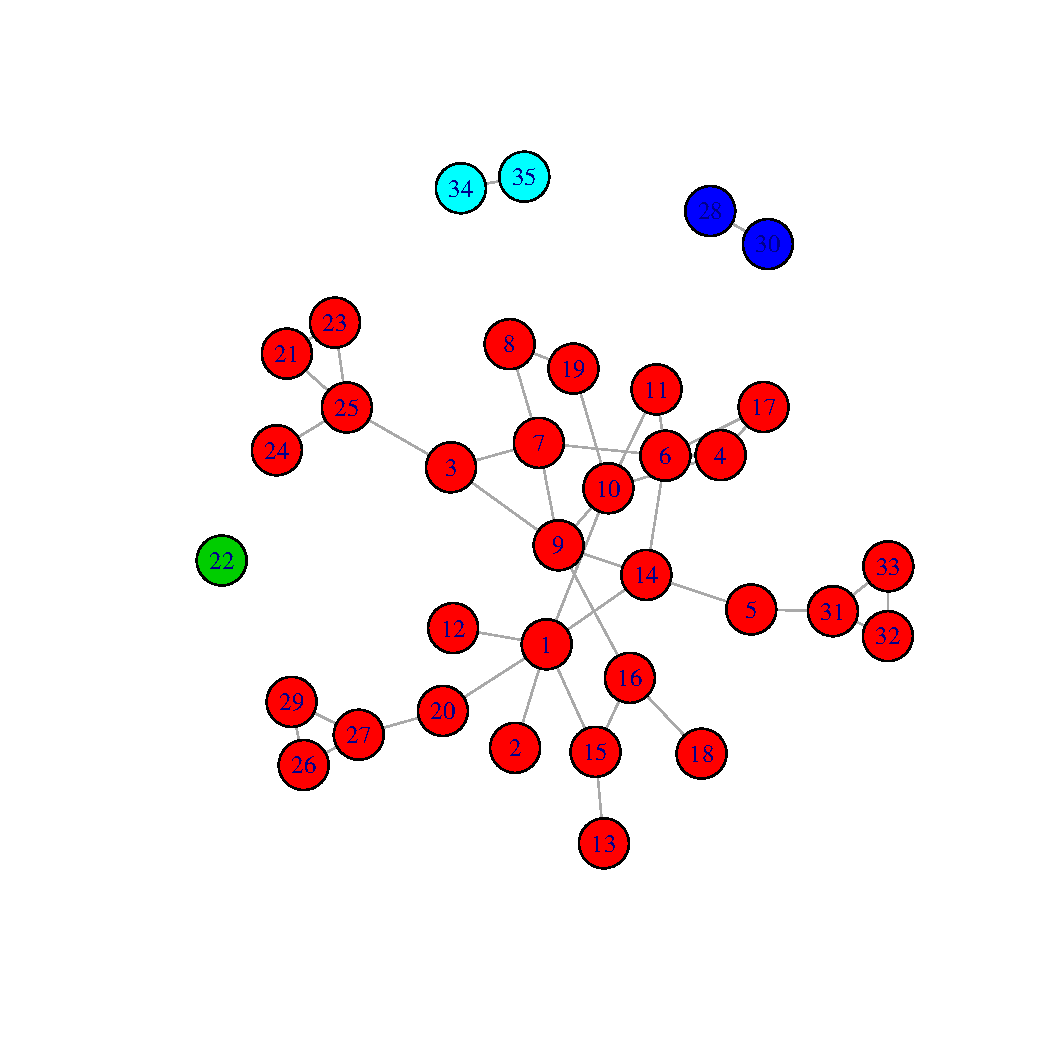
\includegraphics[scale=0.5]{figures/ug.pdf} 
\end{frame}

\begin{frame}
   \frametitle{Weakly Connected Components (Directed Networks)}
   Any two vertices in a component must be connected without regards to direction.
   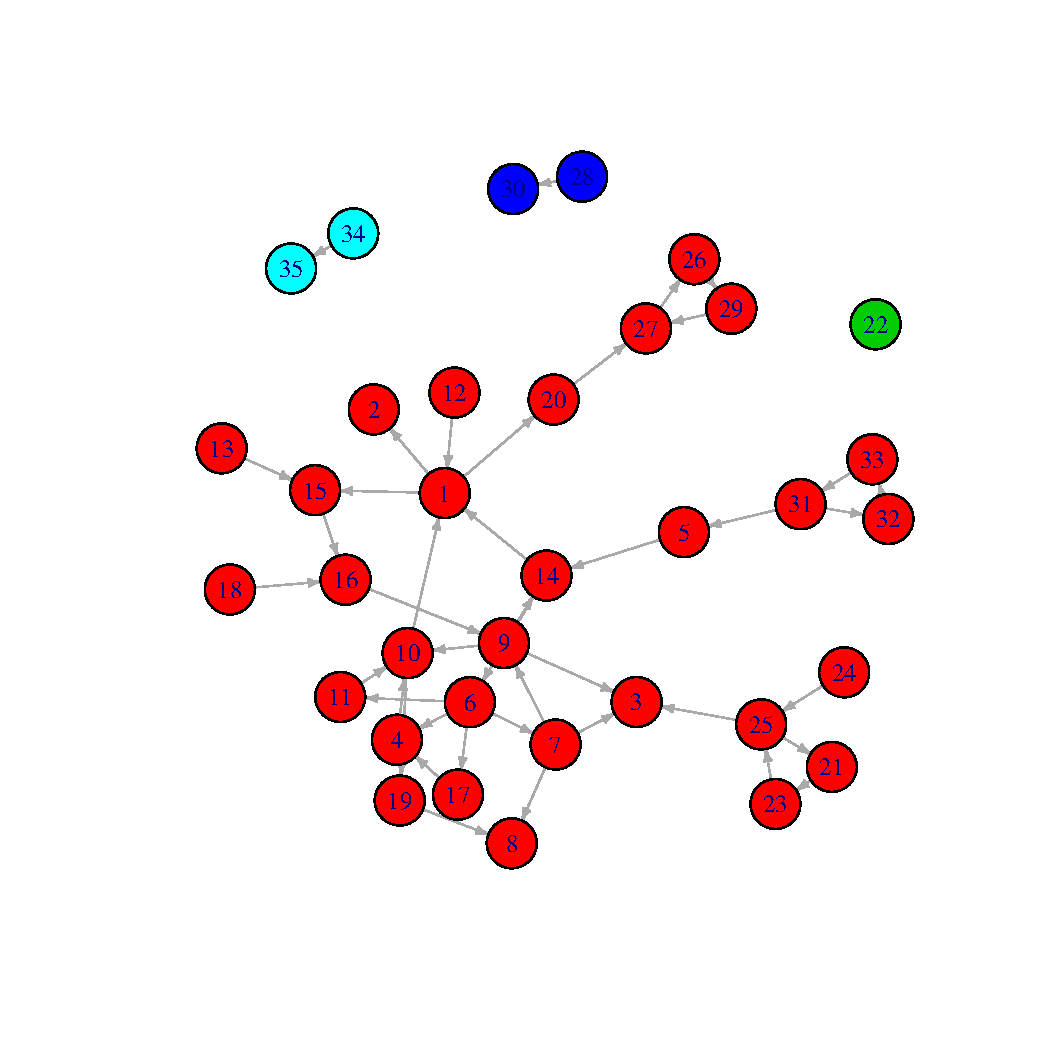
\includegraphics[scale=0.5]{figures/weak_dg.pdf} 
\end{frame}

\begin{frame}
\frametitle{Some Examples of Large Components and Large Weakly 
                 Connected Components}
We typically find that large components are usually more than half of vertex size $(n)$ and not infrequently over 90\% .                
\begin{table}[ht]
\caption{(Table 18.1) Basic stats for some selected networks.
               Where n=no. of vertices, m=no. of edges, c=mean degree, S=\% of largest component.} 
\centering 
\begin{tabular}{r c c c c c}
\hline
Network & Type & n & m & c & S \\  \hline
Marine food web & Directed & 134 & 598 & 4.46 & 1.000 \\
Software pack. & Directed & 1,439 & 1,723 & 1.20 & 0.998 \\
Metabolic & Undirected & 765 & 3,686 & 9.64 & 2.56  \\
Bio. co-auth. & Undirected & 1,520,251 & 11,803,064 & 15.53 & 4.92 \\
Phy. co-auth. & Undirected & 52, 909 & 245,300  & 9.27 & 6.19 \\
Protein int.& Undirected & 2,115 & 2,240 & 2.12 & 6.80 \\
Student dating & Undirected & 573 & 477 & 1.66 & 16.01 \\
\end{tabular}
\end{table}
\end{frame}

\begin{frame} 
   \frametitle{Strongly Connected Components (Directed Networks)}    
   \begin{itemize}
   \item Any two vertices in a component must be connected (directed).
   \item Every strongly connected component generate an {\bf in-component} and an {\bf out-component}.
   \end{itemize} 
\end{frame}

\begin{frame} 
   \frametitle{Example: Strongly Connected Components} 
   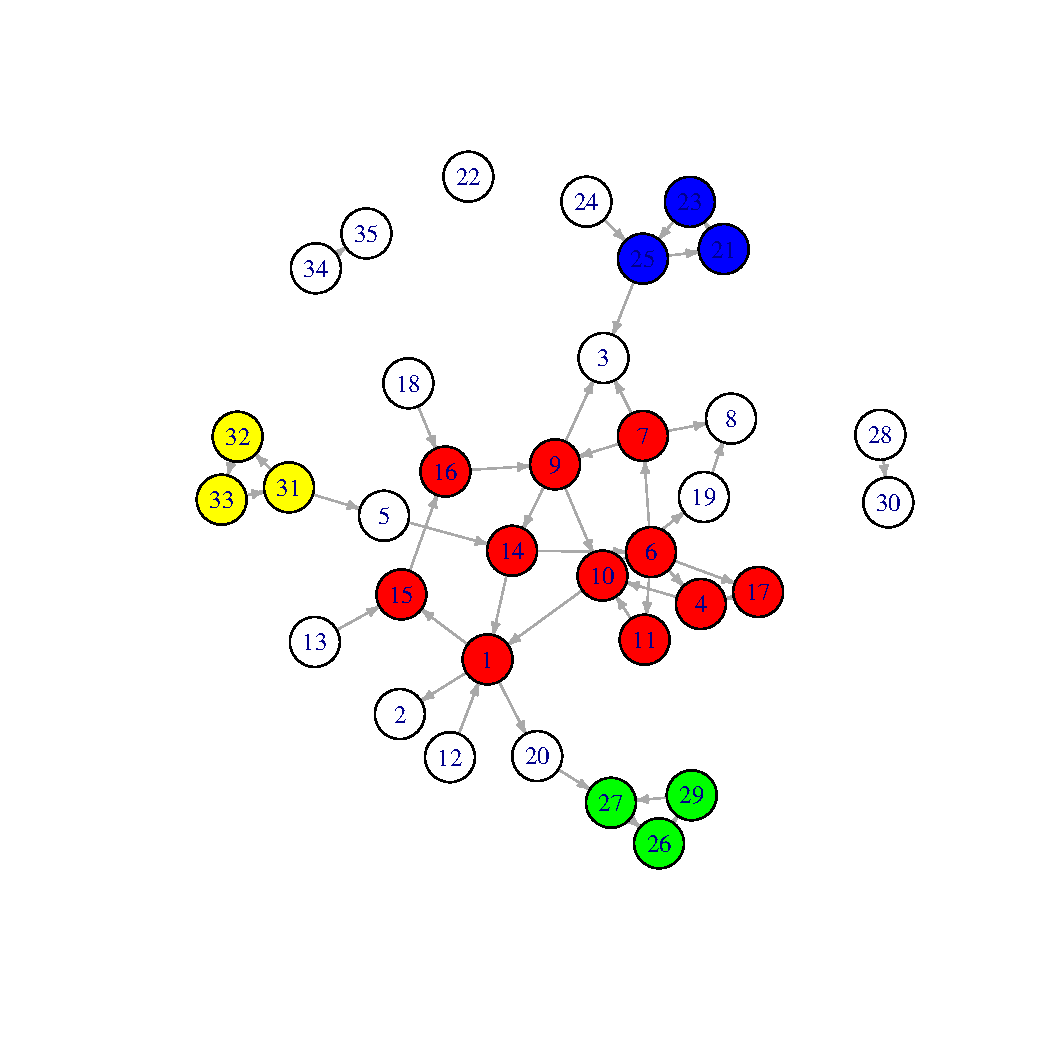
\includegraphics[scale=0.55]{figures/strong_dg.pdf} 
\end{frame}

\begin{frame} 
   \frametitle{The Bowtie Effect} 
   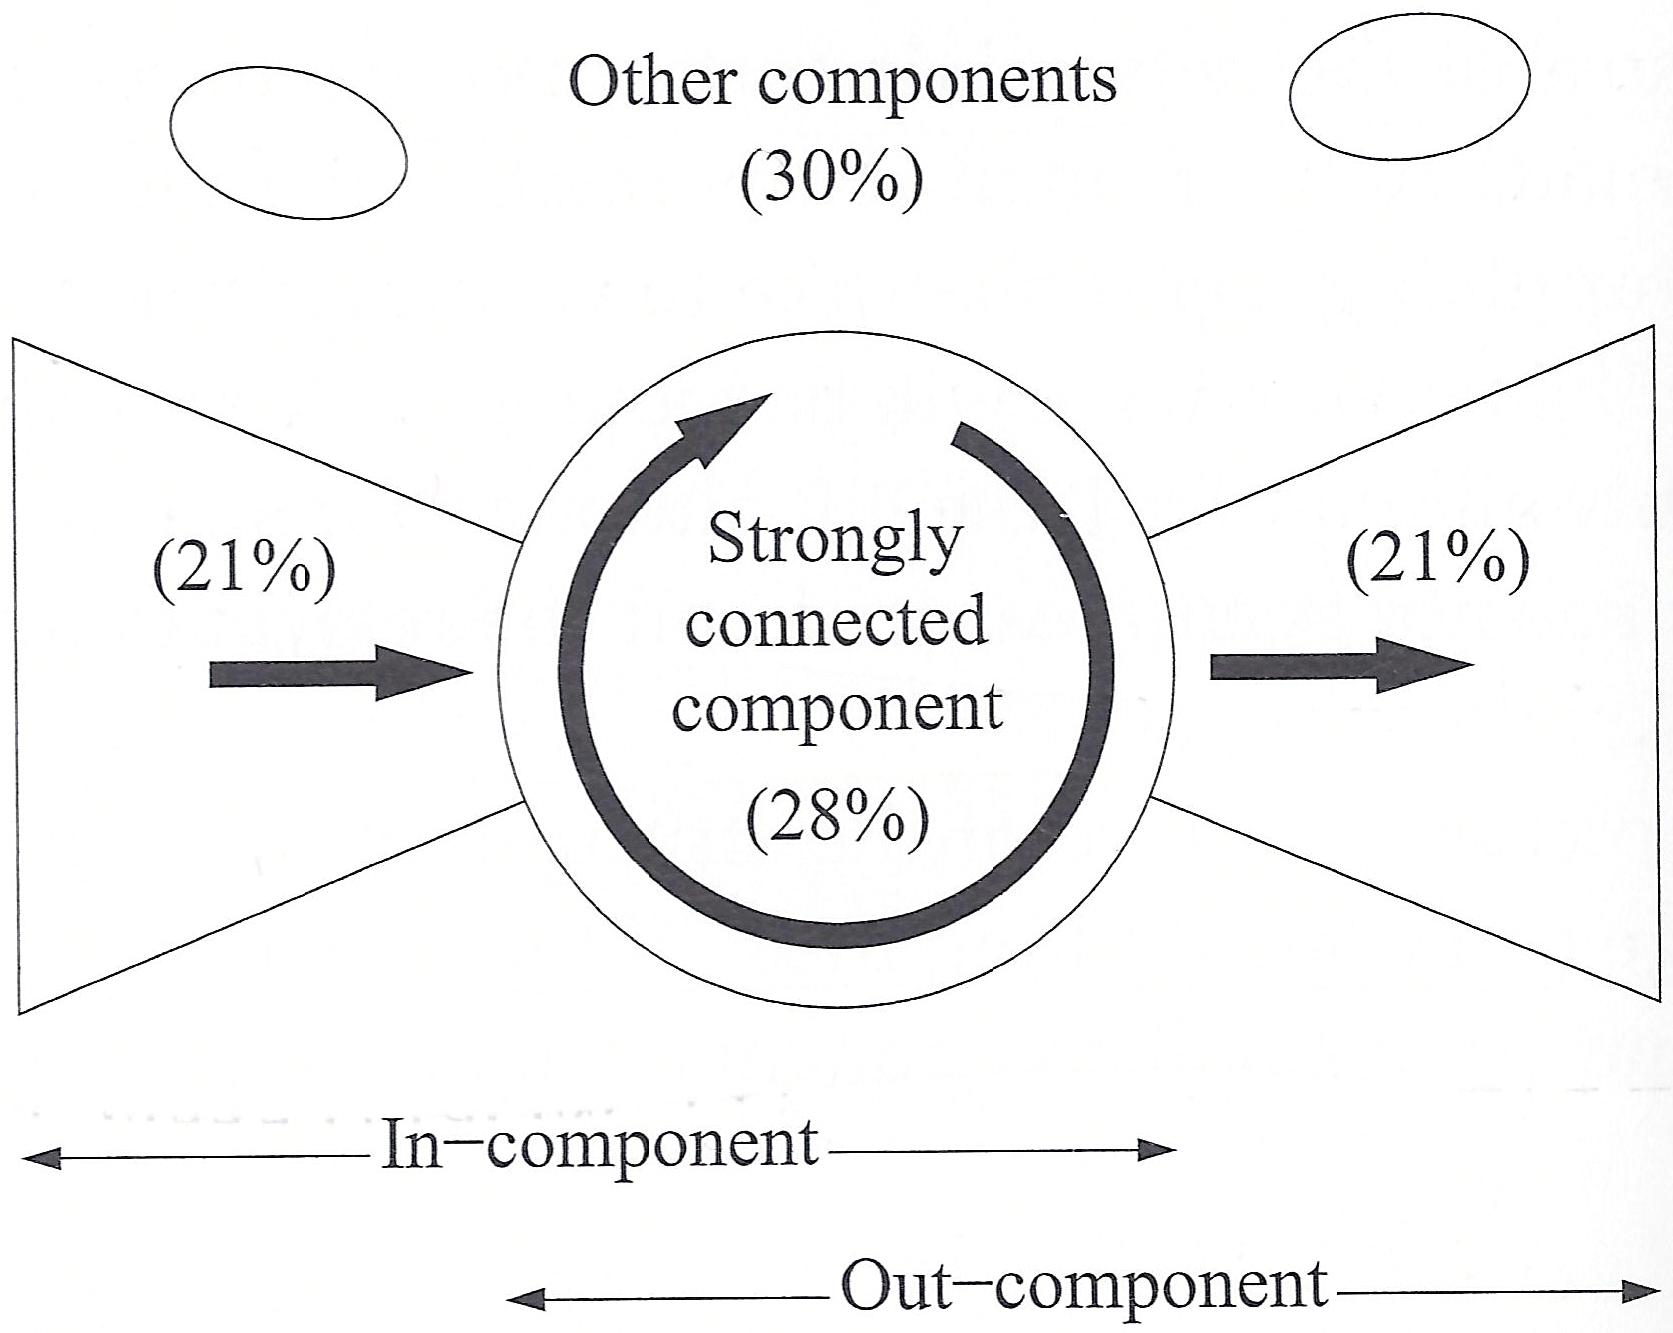
\includegraphics[scale=1.4]{figures/bow_tie.jpg} 
\end{frame}

\begin{frame} 
   \frametitle{The Shortest Path and the Small-World Effect} 
   \begin{itemize}
   \item {\bf Small-world effect}: the observation that in most real world networks the distances between vertices are
   small.\\
   \item Recall: $l_i = \frac{1}{n}\sum_{j} d_{ij}$, where $d_{ij}$ is the shortest path between $i$ and $j$; is the mean
   geodesic distance for vertex $i$.\\
   ${}_{}$\\
   The mean geodesic distance of the network is defined as: $l=\frac{1}{n} \sum_i l_i$.
   \item For random graphs (Erdos-Reyni graphs): $l \propto log(n)$
   \item For scale free networks: $l \propto log(log(n))$\\
   ${}_{}$\\
   (The definition of a scale-free network is below)
   \end{itemize}
\end{frame}


\begin{frame} 
\frametitle{The Shortest Path and the Small-World Effect} 

\begin{table}[ht]
\caption{(Table 18.1) Basic stats for some selected networks. Where l=mean geodesic distance connected vertex pairs.} 
\centering 
\begin{tabular}{r c c c c c}
\hline
Network & Type & n & m & c & l \\  \hline
Metabolic & Undirected & 765 & 3,686 & 9.64 & 2.56  \\
Bio. co-auth. & Undirected & 1,520,251 & 11,803,064 & 15.53 & 4.92 \\
Phy. co-auth. & Undirected & 52, 909 & 245,300  & 9.27 & 6.19 \\
Protein int.& Undirected & 2,115 & 2,240 & 2.12 & 6.80 \\
Student dating & Undirected & 573 & 477 & 1.66 & 16.01 \\
\end{tabular}
\end{table}

\end{frame}


\begin{frame} 
\frametitle{Funneling and the Sociometric Superstars} 
\begin{itemize}
\item (Suggested by Milgram)  {\bf Funneling}: The idea that a given vertex has one or two connecting vertices
that are well connected (i.e. have a high degree). 
\end{itemize}
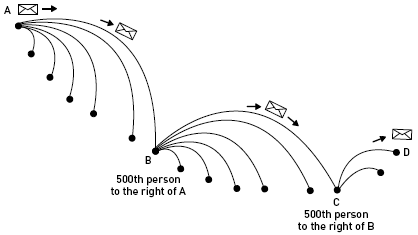
\includegraphics[scale=0.5]{figures/funneling.png} 
\end{frame}

\begin{frame} 
\frametitle{Degree Distributions} 
\begin{itemize}
\item The {\bf distribution of degrees} of a given network is a {\it KEY} fundamental property. 
\item Consider a simple undirected network with vertices, $\{1, 2, \dots, n\}$. 
\item If we pick a vertex $i \in \{1, 2, \dots, n\}$ at random, can we guess what it's degree $k_i$ will be ?\\
${}_{}$\\
No: But we know that it can be any counting number between 0 and $n-1$.\\
${}_{}$\\
Also depending on what natural phenomena the network is describing, we can 
say something sensible (on average).
\end{itemize}
\end{frame}


\begin{frame}
\frametitle{Ways to Characterize A Degree Distribution} 
\begin{table}[ht]
\caption{Degree Distribution in table form} 
\centering 
\begin{tabular}{r c c c c c}
\hline
degree: & 0 & 1 & 2 & $\dots$ & n-1 \\  \hline
probability: & $p_0$ & $p_1$ & $p_2$ & $\dots$ & $p_{n-1}$ 
\end{tabular}
\end{table}
Or
\begin{itemize}
\item Mathematical Function (aka. probability mass function, pmf):\\
${}_{}$\\
$p(k),~~~k=0,1,2, \dots, n-1$. 
\end{itemize}
${}_{}$\\
When $p(k)$ follows the Power Law we say that we have a {\bf scale-network}.\\
${}_{}$\\
When a network has random connections (with a fixed probability of connection) then
we have the {\bf Erdos-Renyi network}. In this case $p(k)$ will follow a Binomial Law 
(usually approximated by a Poisson Law).
\end{frame}

\begin{frame}
\frametitle{Example: Erdos-Renyi (random)}
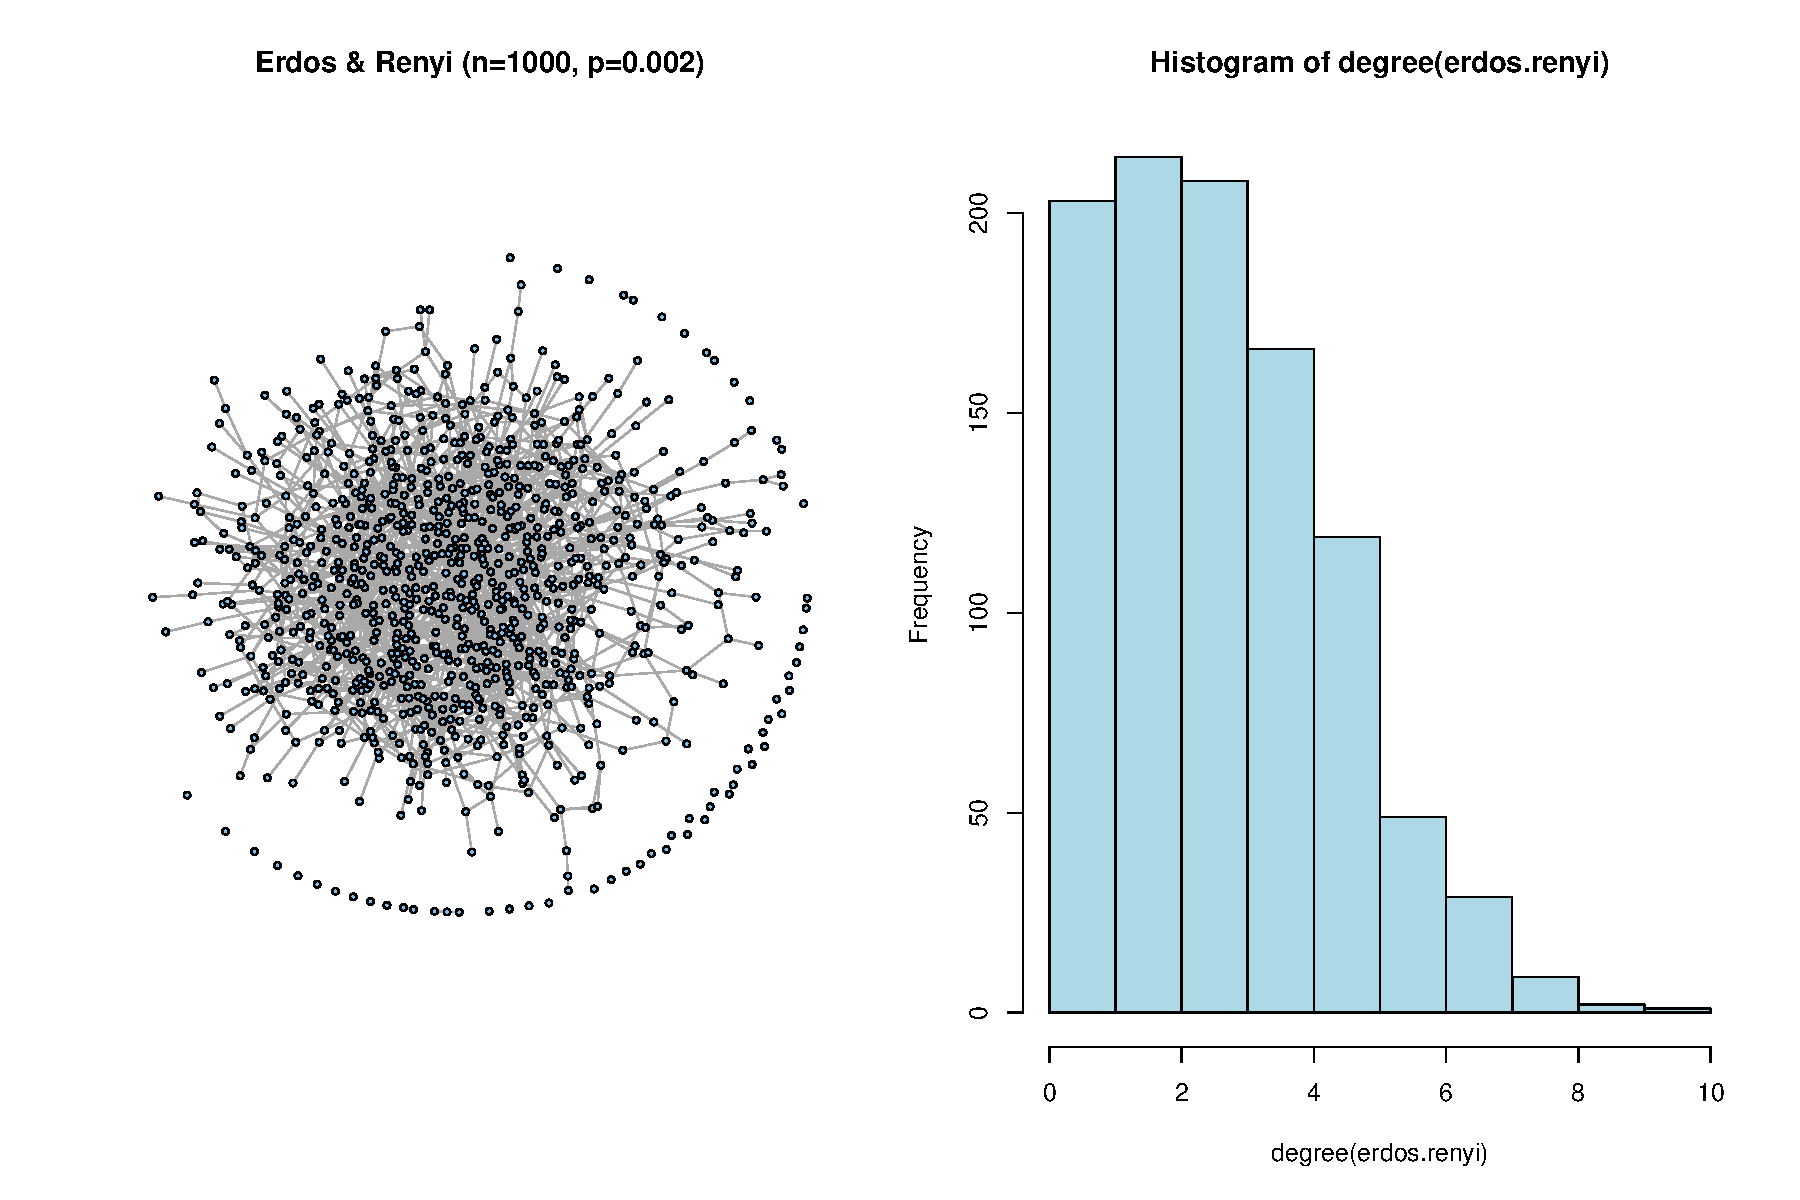
\includegraphics[scale=0.4]{figures/erdos_renyi.pdf} 
\end{frame}

\begin{frame}
\frametitle{Example: Barabasi and Albert (scale free)}
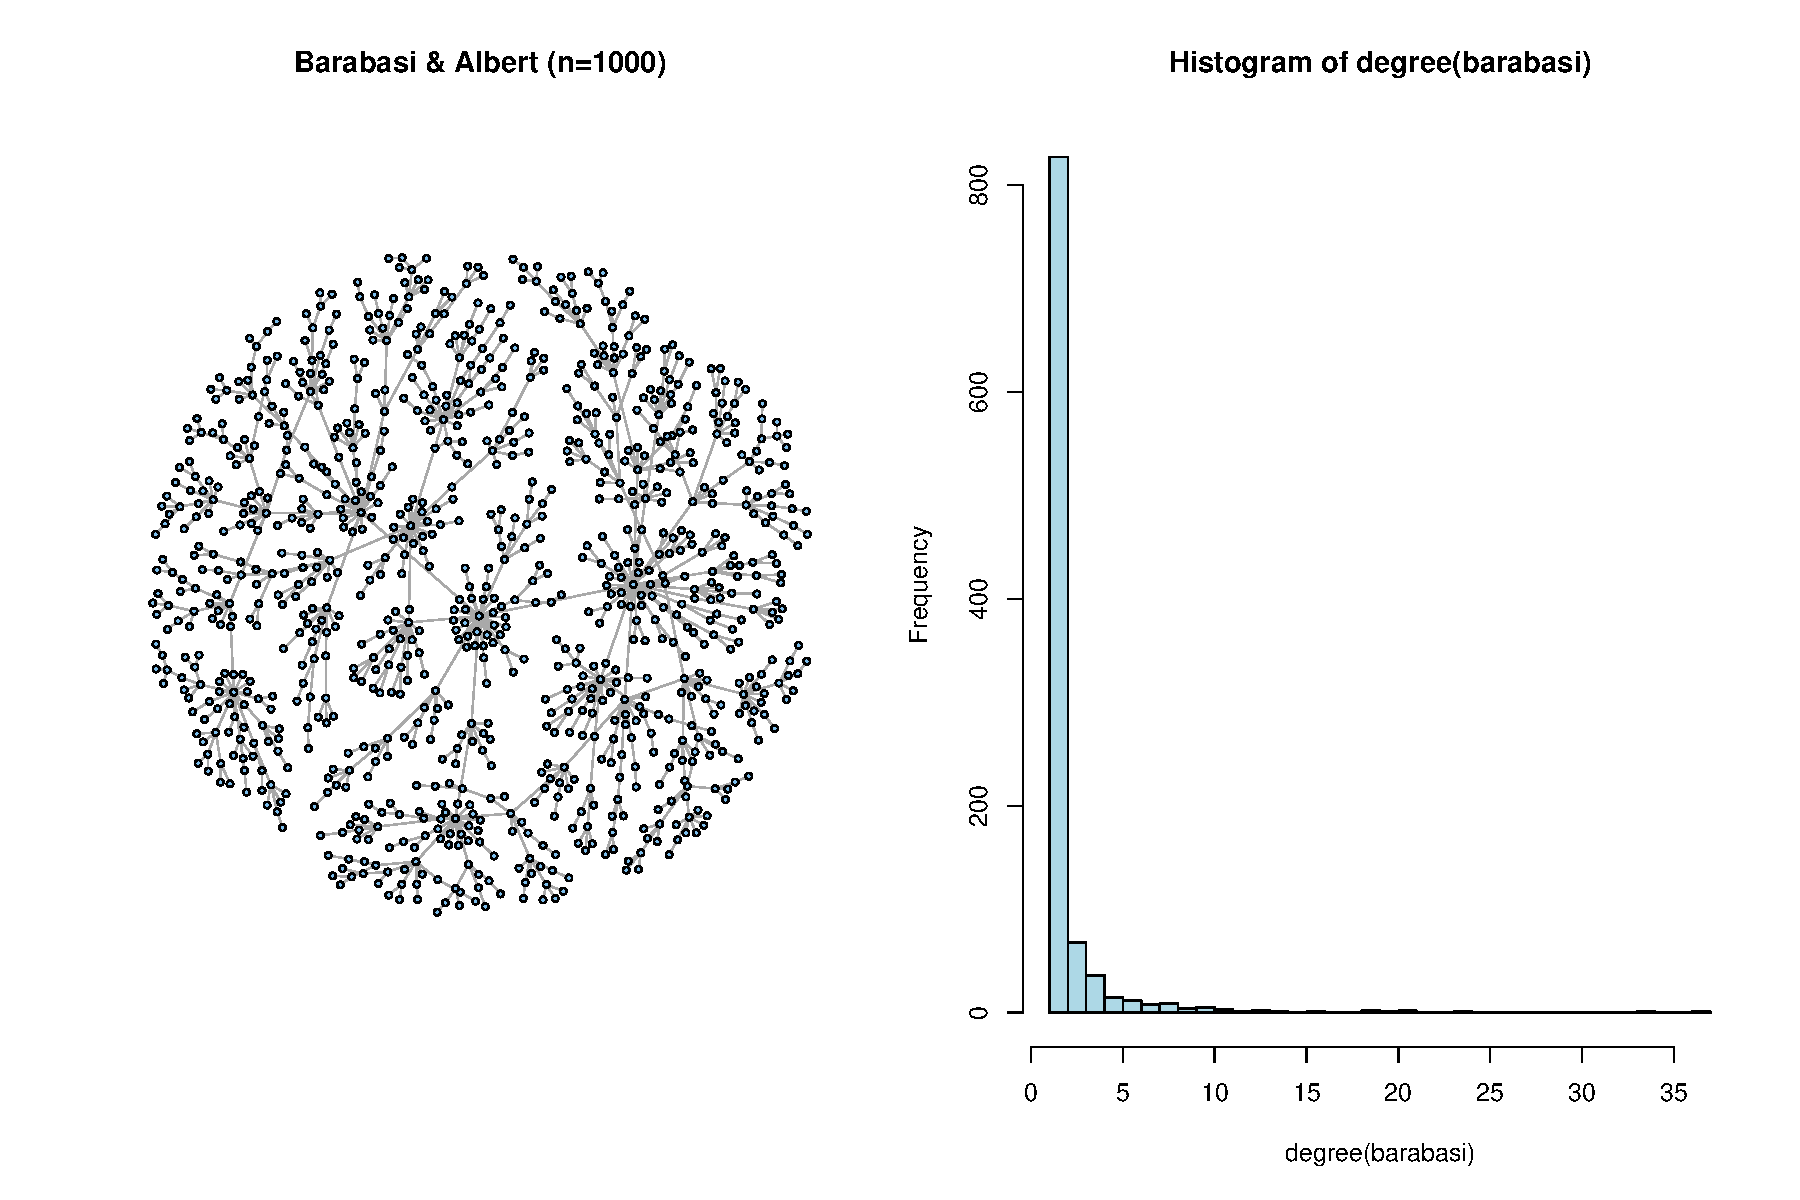
\includegraphics[scale=0.4]{figures/barabasi.pdf} 
\end{frame}

\begin{frame}
\frametitle{Directed Networks}
For directed networks we can talk about the in-degree distribution and the
out-degree distribution, separately.\\
${}_{}$\\
Ideally we would like to know the joint distribution instead. \\
This is an on-going research topic.\\ 
${}_{}$\\
Next time we will look more closely at the Power Law and some of its consequences.
\end{frame}

\end{document}


